\section{Introduction}

Recently linux container clusters draw much attention because they are lightweight, portable and repeatable.
Container clusters are generally more lightweight than Virtual Machine clusters, 
because the containers have seperate execution environment sharing the kernel with host OS. 
They are generally portable, because the process execution environment, especially the file system, are packed
into the tar archives.
Whenever one attempts to run a container, the exact same file systems are restored from the archives, 
even on totally different datacenters. 
This results in a repeatable execution environment.

For Web serviceis, linux containers are attractive becase of the same reasons. 
Furthermore, it is expected that Web systems consisting of container cluster are capable of being easily migrated 
when BCP() and DR() are the requirements. 

The Kubernetes\cite{K8s2017} container cluster management system is one of the prominet candidates
which enble easy container cluster migration.
However it turned out that the kubernetes has issues when it comes to migration, 
because it does not include a load balancer and relies on external load balancers  
which is prepared by cloud providers.
The kubernetes will send a request to an api endpoint of a cloud provider, 
and the cloud provider will automatically setup a load balancer which distribute the traffic from outside to every nodes
 where containers are run on. Then the traffic is forwarded again using iptables DNAT\cite{MartinA.Brown2017,Marmol2015} rule with the round-robin manner. 

This does not necessarily work for all cloud provider nor for on-premise datacenters.
There exist environments
where there is no load balancer which is supported by the Kubernetes.

When the Kubernetes container cluster management system is deployed on such environment,
there will be a need for a static and adhoc routing setups for traffic from outside.

In this paper, we propose a software load balancer deployed as a container in Kubernets system. 
We will implement ipvs\cite{Zhang2000} layer 4 load balancer as a container and 
investigate the feasibility of such load balancer by comparing the perfomance with iptables DNAT and nginx proxy.

We will also investigate appropriate network settings which enable such load balancers to work properly.

The rest of the paper is organized as follows.
The section \ref{Related Work} highlights related work specifically those deal with container cluster migration, 
software loadbalancer containerization or a loadbalancer related tools in the context of container. 
The section \ref{Load balancers in Kubernetes cluster} will explain the problem of the exsisting architecture and propose our solution.
In the section \ref{Performance Measurement}, experimental conditions and the parametes we used in the experiment are described in detail.
We will show the result of experiment and disscuss the characteristics in the section \ref{Result and Discussion} 
followed by the conclusion in the section~\ref{Conclusions}.
  

\section{Related Work}\label{Related Work}
This section highlights related work specifically those deal with container cluster migration, 
software loadbalancer containerization or a loadbalancer related tools in the context of container. 

Some developers of the kubernetes are trying to add federetion\cite{K8sFederation2017} capability 
where multiple Kubernetes clusters are deployed on multiple cloud providers or on-premise datacenters 
and are managed via federation api server. However, how each of Kubernetes clusters is run on different type of cloud providers
or in on-premise datacenters, especially when the load balancers of such environments are not supported by the Kubernetes, 
is out of the scope of the project. 
   
As far as the containerization of a load balancers are concerned, there are following related works:
Nginx-ingress\cite{Pleshakov2016,NginxInc2016} utilizes the ingress\cite{K8sIngress2017} capability of the Kuberentes, 
and implements contanerized nginx proxy as a load balancer. The nginx itself is famous as a high performance web server program,
which also has the functionality of layer 7 load balancer. The nginx is capable of handling TLS encryption and also capable of  
URI based switching. However the flip side of these is that it is much slower than layer 4 switching.
The upper bound of the performance of the nginx as a load balancer will not exceed that as a single web server serving lightweight web pages. 
Therefore it is meaningless to use the nginx as a load balancer in such cases.
 
The kube-keepalived-vip\cite{Prashanth2016} project is trying to use the linux kernel's loadbalancer capability, 
called ipvs\cite{Zhang2000} by containerizing the keepalived\cite{ACassen2016} and ipvs. 
The keepalived container is using the daemonsets\cite{K8sDaemonsets2017} capability of the Kubernetes, 
where the container is run on every node.
This work is very similar to our proposal in the sense that it uses keepalived and ipvs in container. However it does not provide 
per container cluster load balancer which is portable among different cloud providers.   
Our proposal is to provide a load balancer that is configurable and deployable at user's will,
 as a part of container cluster itself not as a port of the infrastructure.  

The swarm mode of the dokcer\cite{DockerCoreEngineering2016,DockerInc2017} also uses ipvs for internal load balancing,
however it is also considered as built-in load balancer functionality of the docker, 
and is not different from our proposal.

There are several other projects where an effort to utilize ipvs in the context of container environment.
The gorb\cite{Sibiryov2015} and the clusterf\cite{Aaltodoc:http://urn.fi/URN:NBN:fi:aalto-201611025433} are daemons 
which setups ipvs in the kernel inside docker container. They utilize information about runnning container inside key-value storages
like the etcd\cite{CoreOSEtcd} and the consul\cite{HashiCorpConsul}. 
These has the similar functionality which is realized by a combination of keeapalived and the kubernetes ingress controller in our proposal.
These may be usable in our environment in future, but that is beyond the scope of this paper.

The contribution of the paper are followings: 
1) We propose a portable load balancer as a container for the kuberbetes cluster 
that is deployable on almost any cloud provider or on on-premise datacenters.
2) We discuss feasibility of the above by quantitativly measuring the performance.


\section{Load balancers in Kubernetes cluster}\label{Load balancers in Kubernetes cluster}

\subsection{Conventional Architecuture}

\begin{figure}
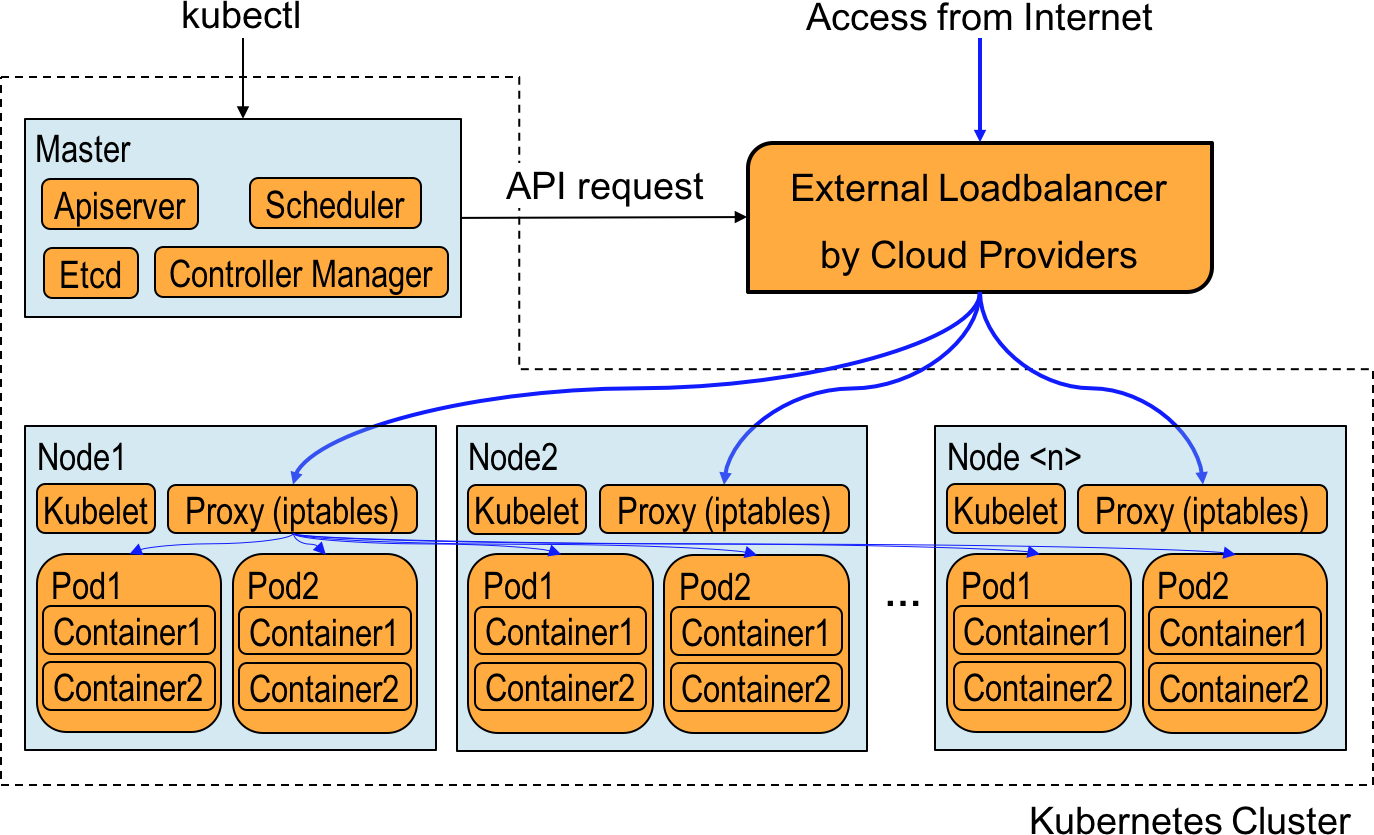
\includegraphics[width=\columnwidth]{Figs/K8sConventional}
\caption{Conventional Architecture of A Kubernetes cluster.}
\label{fig:K8sConventional}
\end{figure}

The kubernetes container management system has an issue when it is used in outside of recommended cloud providers e.g. GCP or AWS.
Figure~\ref{fig:K8sConventional} shows a exemplified Kubernetes cluster.
The kubernets cluster typically consists of master servers and node servers.
On the master servers daemons that control the Kubernetes cluster are typically deployed. 
These daemons include, apiserver, scheduler, controler-manager and etcd. 
On the node servers, the kublet daemon will run pods, depending the PodSpec information obtained from the apiserver on the master servers.
A pod is a group of containers which share the net name space and cgroups, and is the basic execution unit in the Kubernets cluster.

When a service is created, the masters will send out request to cloud providers API endpoints, to set up external load balancers.
The proxy daemon on the node servers will also setup iptables DNAT\cite{MartinA.Brown2017} rules, 
which distributes the inbound traffic to the existing pods.

The traffic from the internet will be distributed by the external load balancer to node servers evenly, 
then it will be distributed again by the DNAT rules on the node serves to designated pods. 
The returning packets will follow the exact same route as the incoming ones.

The problems of this architecture are the following: 
1) Having external load balancers whose apis are supported by the Kubernetes daemons is the prerequisite. 
There are many cloud providers where the api of load balancers is not supported by Kubernetes. 
There are many load balancers which dose not even have APIs that is usable by Kubernets, for on-premise datacenters.  
In such cases, one could manually setup the routing table on a gateway to one of the node servers, 
then the traffic will be distributed by the DNAT rules on the node to designated pods.
However this is far from convenient.
2) Distributing the traffic twice, firstly on the external load balancers and secondary on each node, 
will complicate the route a packet follows. Imagine the situatiuon, where the DNAT table on one of the node servers malfunctions.
In such case, you will only observe occasional timeouts. It is very difficult to find out which node server malfunctions.   

\subsection{Proposed Architecture}

\begin{figure}
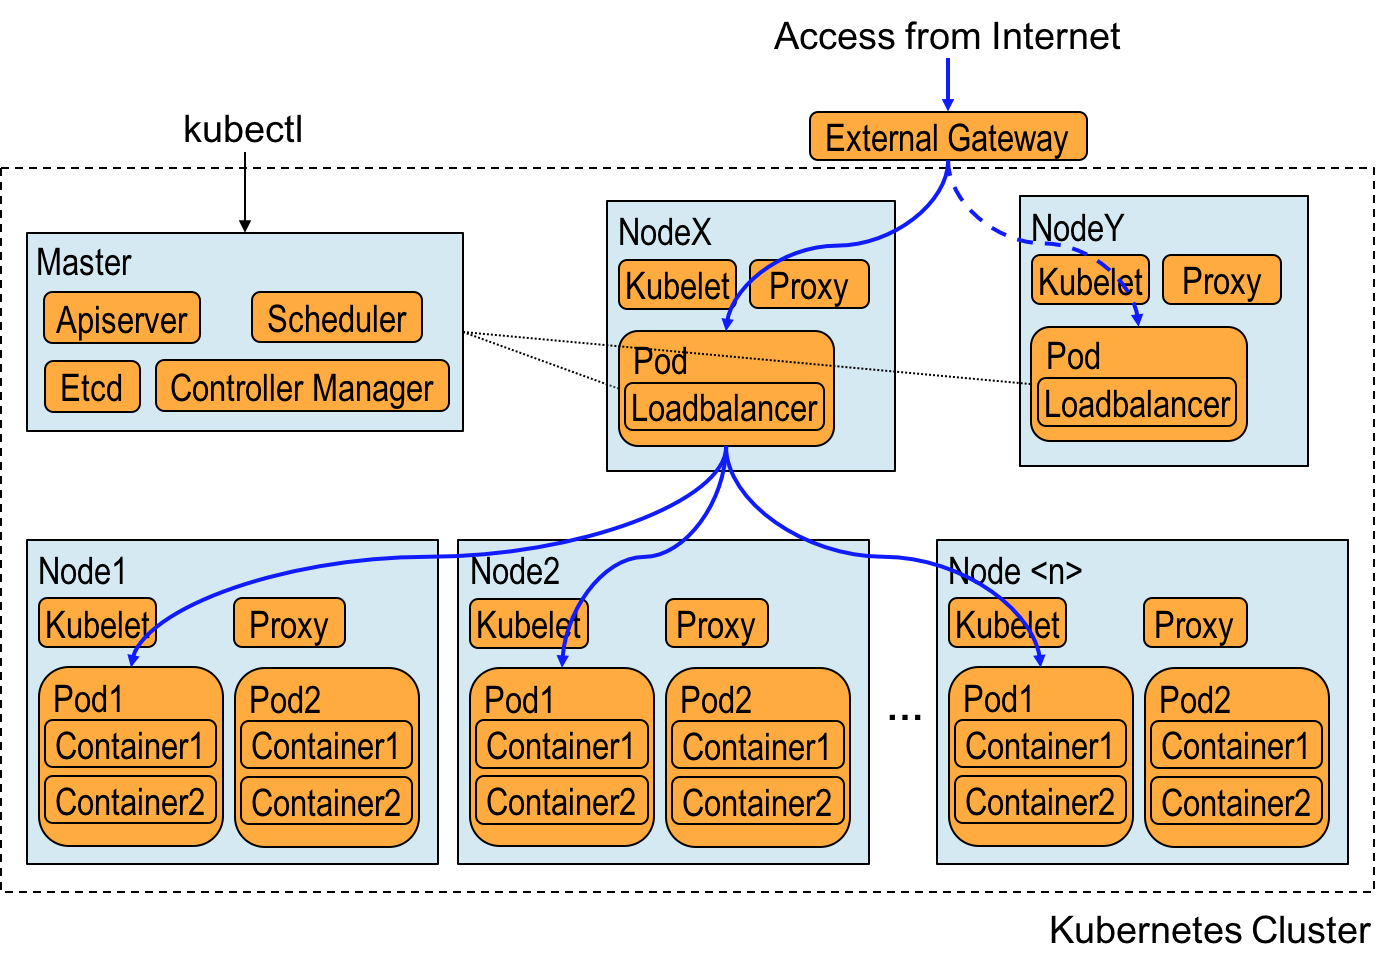
\includegraphics[width=\columnwidth]{Figs/K8sProposed}
\caption{A Kubernetes cluster with proposed load balancer.}
\label{fig:K8sProposed}
\end{figure}

Figure~\ref{fig:K8sProposed} shows the proposed architecture of the Kubernetes cluster, 
which has following characteristics:
1) Each load balancer itself is run as a pod by the Kuberenets system. 
2) There exist multiple load balancers for redundancy. 
3) Configuration of the load balancers are dynamically changed depending on the information of running pods responsible for services.

By following these architecture, we can resolve the problems of conventional architecture.
Since load balancer itself is containerized, it can be run on any environment including on-premise datacenters.
And because it only distribute traffic only once on the load balancer, it is relatively easy to find malfunctions.

In this paper, we propose a containerized software load balancer. 
Specifically we will implement a container which setup Linux kernel's load balancer functionality, 
ipvs inside the container's net name space.
We also discuss the feasibility of the proposed load balancer by comparing the performance with existing iptables and nginx based load balancer. 


\subsection{Implementation}\label{Implementation}

\begin{figure}
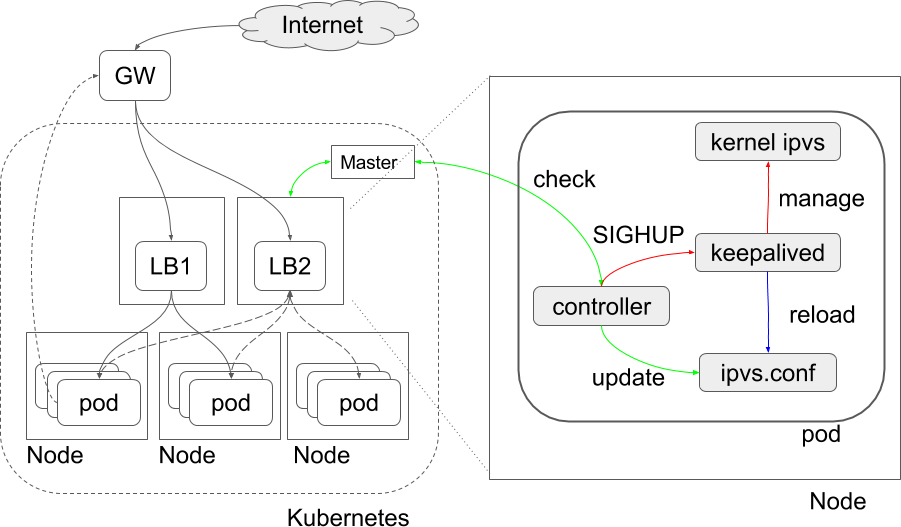
\includegraphics[width=\columnwidth]{Figs/ipvs-ingress-schem}
\caption{Implementation}
\label{fig:ipvs-ingress-schem}
\end{figure}

Figure~\ref{fig:ipvs-ingress-schem} show the schematic diagram of a container that functions as a load balancer.
Inside the container, two daemons, controller and keepalived are run.
The keepalived is a program which modifies linux kernels ipvs rules depending on the configuration file, ipvs.conf.
The keepalived is also capable of healthchecking the liveliness of realserver, 
which is a combination of IP address and port number of the target pods. 
If the healthcheck to a real server fails, the keepalived will remove that real server from the ipvs rules.

The controller monitors information of runing pods of a service in the Kuberenetes cluster by consulting the apiserver on the master server.
Whenever pods are created or deleted, it will automatically regenerate appropriate ipvs.conf and issue SIGHUP to the keepalived.
Then the keepalived will reload the ipvs.conf and modify the kernel's ipvs rules.  

The actual controller\cite{ktaka_ccmp_2017_826894} has been implemented using ingress controller\cite{K8sIngress2017} scheme of the Kubernetes.
By importing existing Golang package, ”k8s.io/ingress/core/pkg/ingress”,
we only needed 120 lines of code.  

In this way, the ipvs's balancing rules inside linux kernel are maintained so that it could distribute the incoming traffic only to the living pods.

In order to let the kernel to load required kernel modules inside a container, 
we needed to add the CAP\_SYS\_MODULE capability to the container, and also needed to mount the /lib/module of the node's file system 
on the container's file system.   

In order to let the keepalived manipulate kernel's ipvs rules, 
we needed to add CAP\_NET\_ADMIN capability to the container.

There is a explanation in a reference\cite{Pai2016} about some of the capbilities that is dropped inside docker containers.

\begin{figure}
\begin{minipage}{0.8\columnwidth}
\begin{verbatim}

virtual_server fwmark 1 {
  delay_loop 5
  lb_algo lc
  lb_kind NAT
  protocol TCP
  real_server 172.16.21.2 80 {
    uthreshold 20000
    TCP_CHECK {
      connect_timeout 5
      connect_port 80
    }
  }
  real_server 172.16.80.2 80 {
    uthreshold 20000
    TCP_CHECK {
      connect_timeout 5
      connect_port 80
    }
  }
}

\end{verbatim}
\end{minipage}
\caption{An example of ipvs.conf}
\label{fig:ipvs.conf}
\end{figure}

\begin{figure}
\begin{minipage}{\columnwidth}
\small
\begin{verbatim}

# kubectl exec -it ipvs-controller-4117154712-kv633 -- ipvsadm -L
IP Virtual Server version 1.2.1 (size=4096)
Prot LocalAddress:Port Scheduler Flags
  -> RemoteAddress:Port Forward Weight ActiveConn InActConn
FWM  1 lc
  -> 172.16.21.2:80      Masq    1      0          0         
  -> 172.16.80.2:80      Masq    1      0          0

\end{verbatim}
\end{minipage}
\caption{An example of ipvs balancing rules}
\label{fig:ipvs rule}
\end{figure}

Figure~\ref{fig:ipvs.conf} shows an example of ipvs.conf file generated by the controller. 
Shown in Figure~\ref{fig:ipvs rule} is the correspoding ipvs's balancing rules.
We can see that the packet with {\tt fwmark=1}\cite{BertHubert2002} is distributed to 172.16.21.2:80 and 172.16.80.2:80 
using masquarade mode(Masq)\cite{Zhang2000} and least connection(lc)\cite{Zhang2000} balancing algorithm.   

\section{Performance Measurement}\label{Performance Measurement}

We carried out performance measurment of the proposed load balancer using benchmark program called, wrk\cite{Glozer2016}.
We also measured performance of iptables's DNAT load balancing functionality and nginx layer 7 load balancer, for comparison.

When creating Kubernetes cluster, an overlay network\cite{Sill2016,Marmol2015} is often used. 
Among available overlay networks, the flannel\cite{CoreOSFlannel} is a popular one.
We compared each of the three backends\cite{CoreOSFlannelBackend}, {\it i.e.} operating modes of the flannel for the benchmark of the load balancers.

It is known that distributing the handling of interrupts from the NIC 
and the following IP protocol processing, among multiple cores are important.

In order to derive best performance, we also investigated how this would affect the performance of load balancers.

\subsection{Benchmarking method}

\begin{figure}
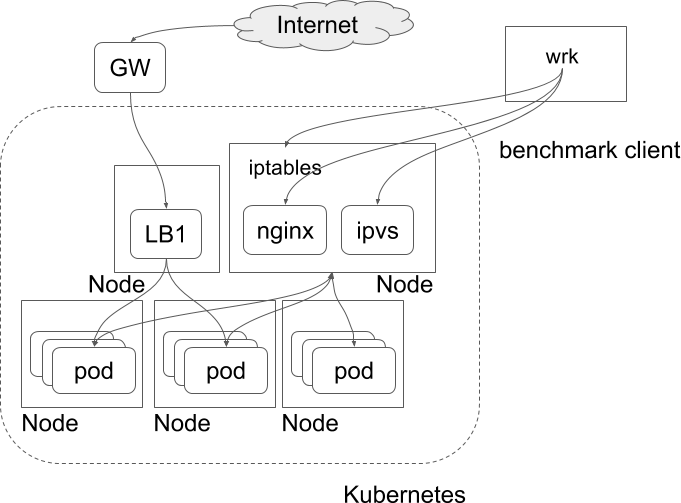
\includegraphics[width=\columnwidth]{Figs/benchmark-schem}
\caption{Benchmark setup}
\label{fig:benchmark-schem}
\end{figure}

Using wrk, we measured performance of the load balancers.
Figure~\ref{fig:benchmark-schem} shows schematic diagram of the experimental setups.

Having deployed pods running nginx web servers which returns IP address of the pod itself,
we set up the ipvs, iptables and nginx load balancers on one of the node servers. 

The HTTP GET requests are sent out from the wrk on the client machine toward the node servers.
The destination IP address and port number is chosen 
depending on the type of the load balancer on which the measurment is performed.
The load balancer on the node server then distribute the requests to pods.
Each pod will return HTTP responses to the load balancer and the load balancer will then return the respose to the client.

The number of responses received by the wrk on the client is counted, 
then the (normally processed) request/sec is obtained. 

\begin{figure}
\begin{minipage}{\columnwidth}
\small
\begin{verbatim}

# kubectl exec -it ipvs-controller-4117154712-kv633 -- ipvsadm -L
IP Virtual Server version 1.2.1 (size=4096)
Prot LocalAddress:Port Scheduler Flags
  -> RemoteAddress:Port Forward Weight ActiveConn InActConn
FWM  1 lc
  -> 172.16.21.2:80      Masq    1      0          0         
  -> 172.16.80.2:80      Masq    1      0          0

\end{verbatim}
\end{minipage}
\caption{An example of ipvs balancing rules}
\label{fig:ipvs rule}
\end{figure}




\subsection{Overlay network}

\begin{figure}
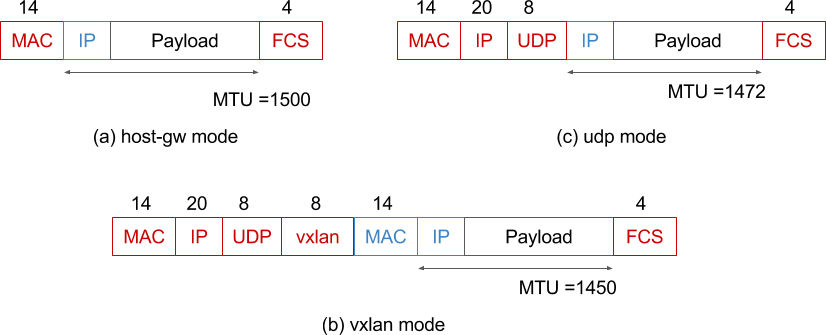
\includegraphics[width=\columnwidth]{Figs/flannel-packet-diagram}
\caption{frame diagram}
\label{fig:flannel-packet-diagram}
\end{figure}


\subsection{Distributed packet handling}

\section{Result and Discussion}\label{Result and Discussion}

\begin{figure*}
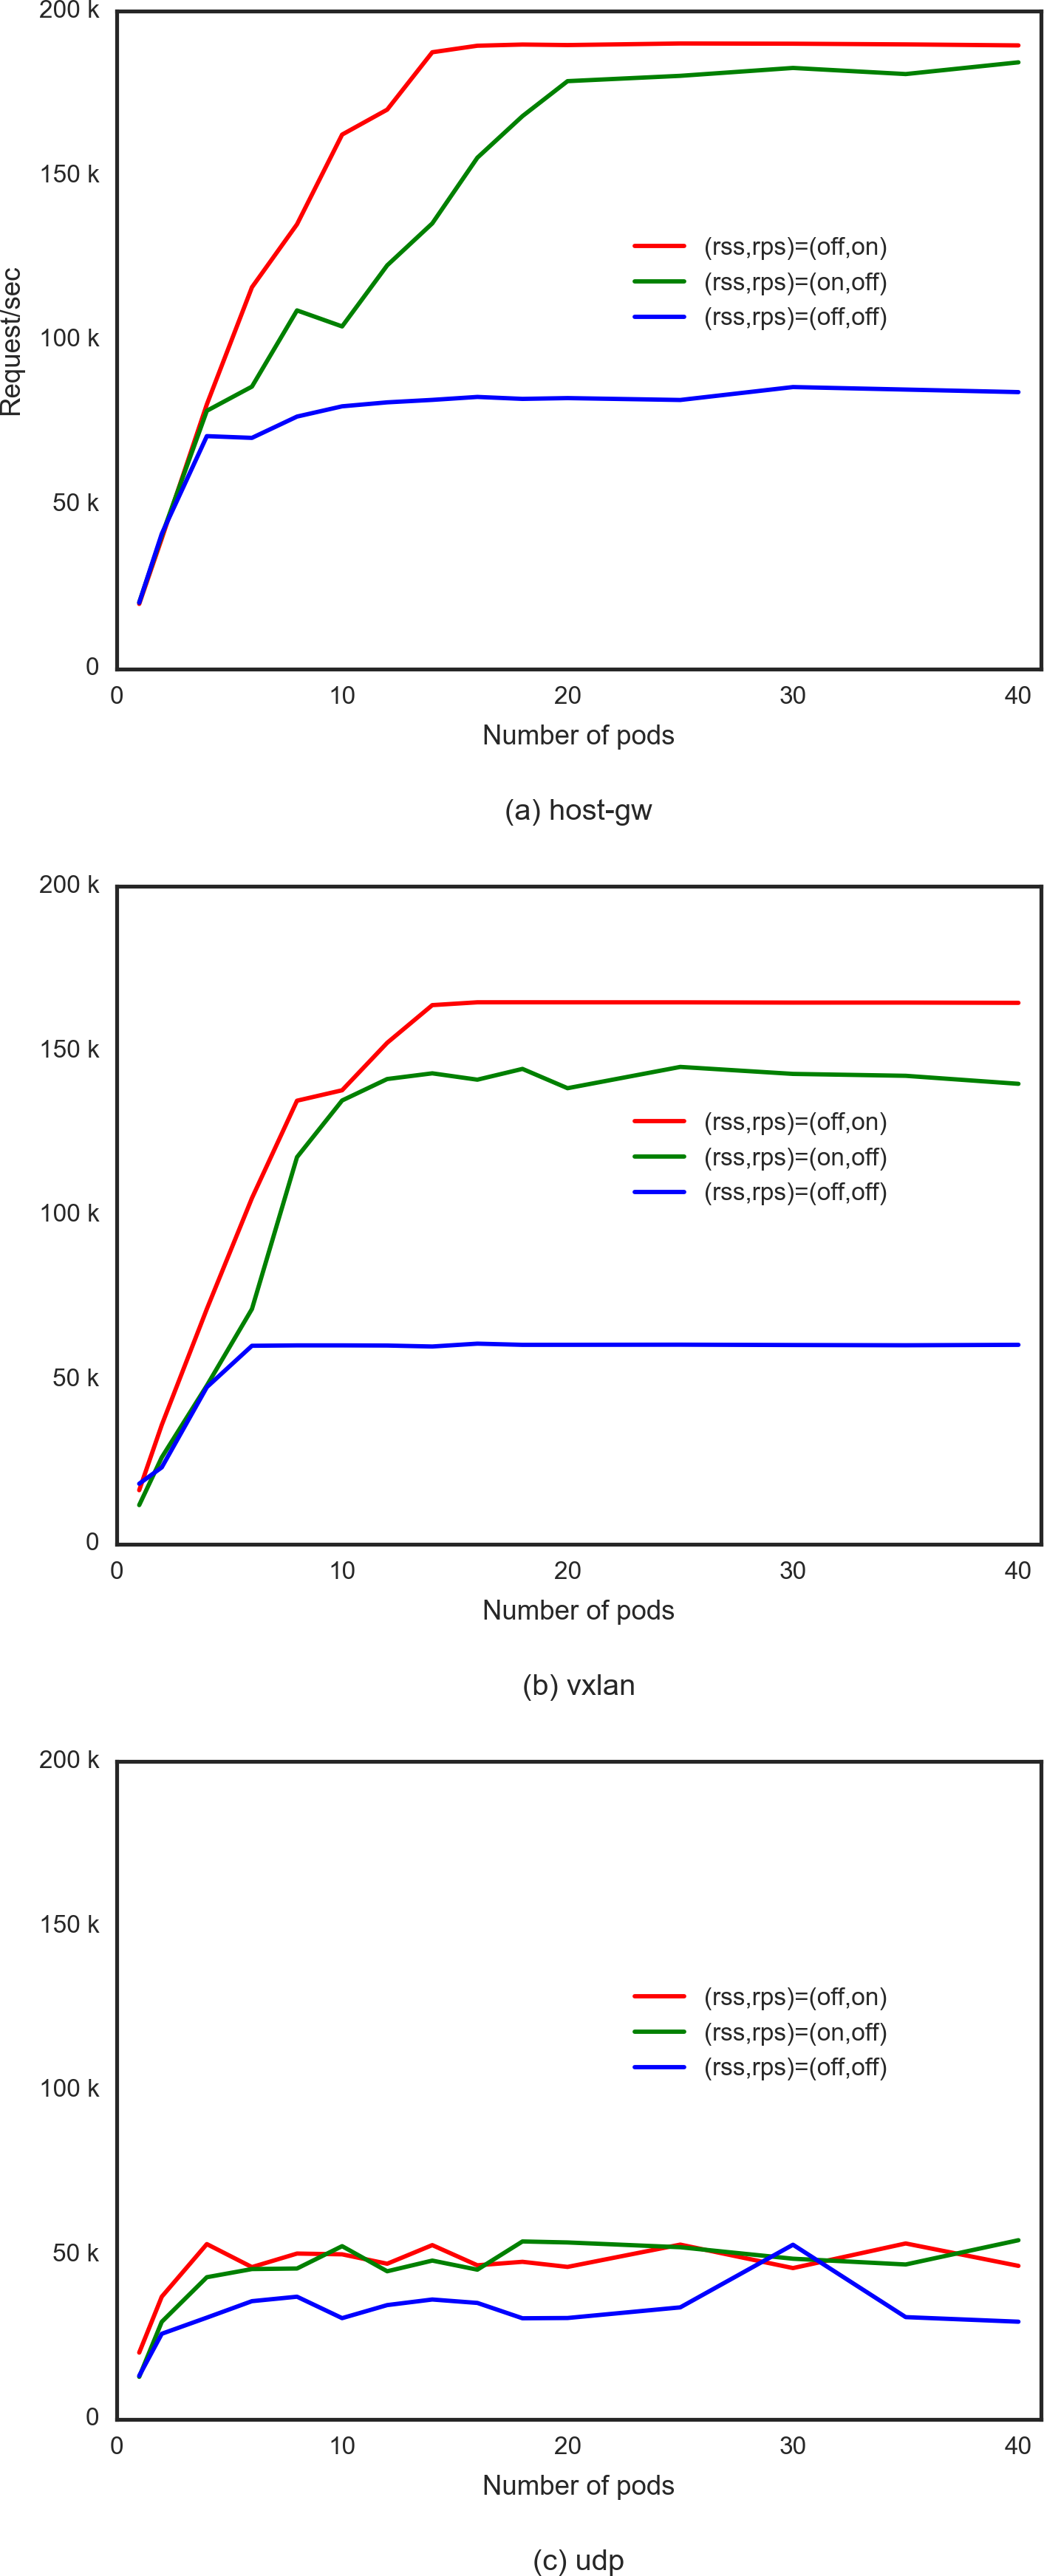
\includegraphics[width=\textwidth]{Figs/iptables_3figs}
\caption{iptables results}
\label{fig:iptabls3figs}
\end{figure*}

\begin{figure*}
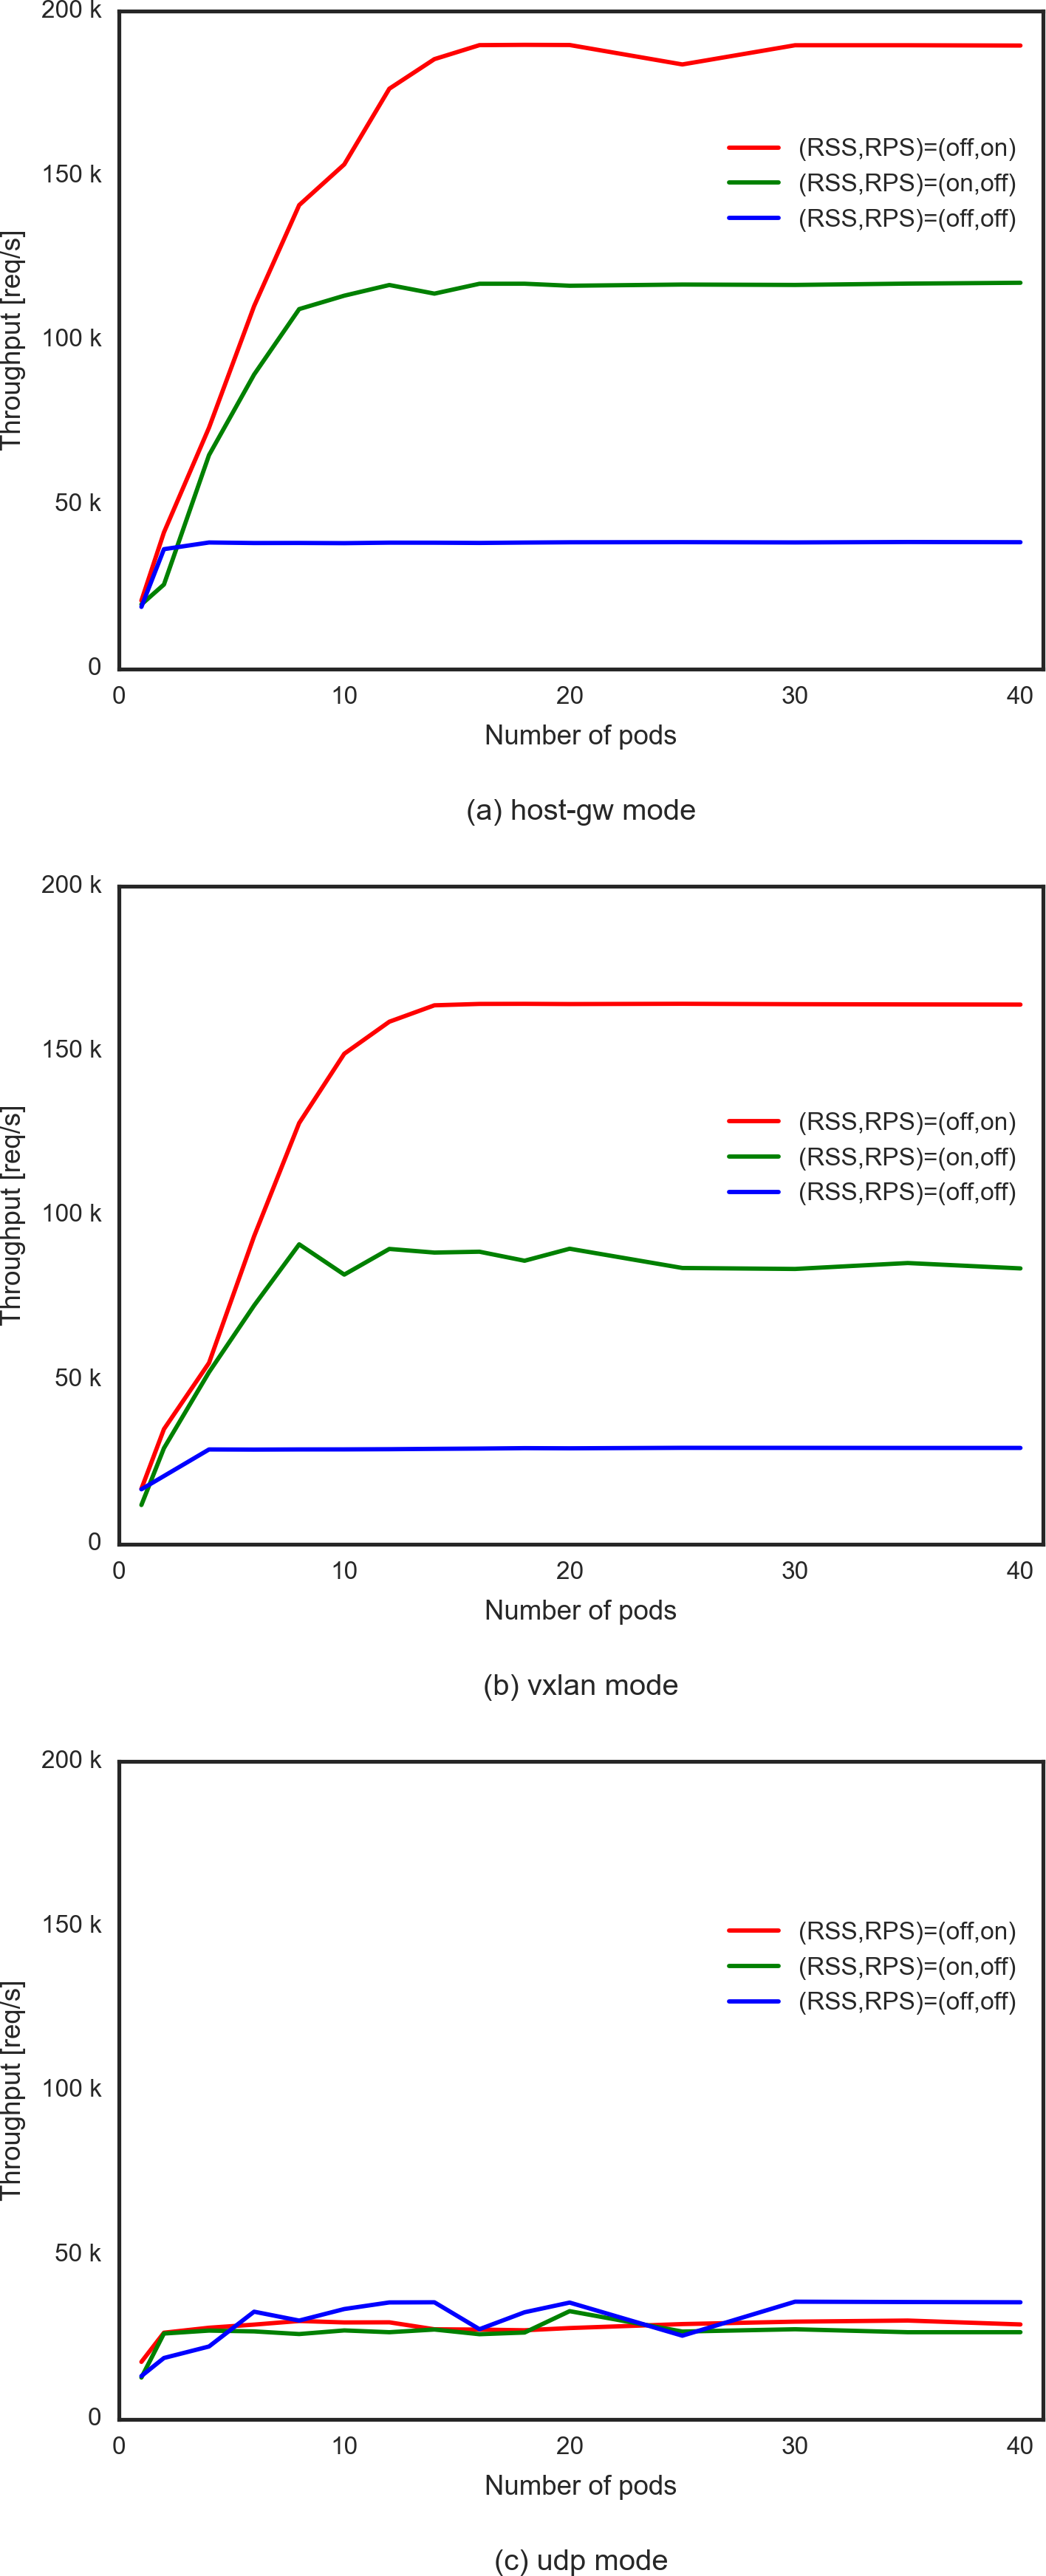
\includegraphics[width=\textwidth]{Figs/ipvs_3figs}
\caption{ipvs results}
\label{fig:ipvs3figs}
\end{figure*}

\begin{figure}
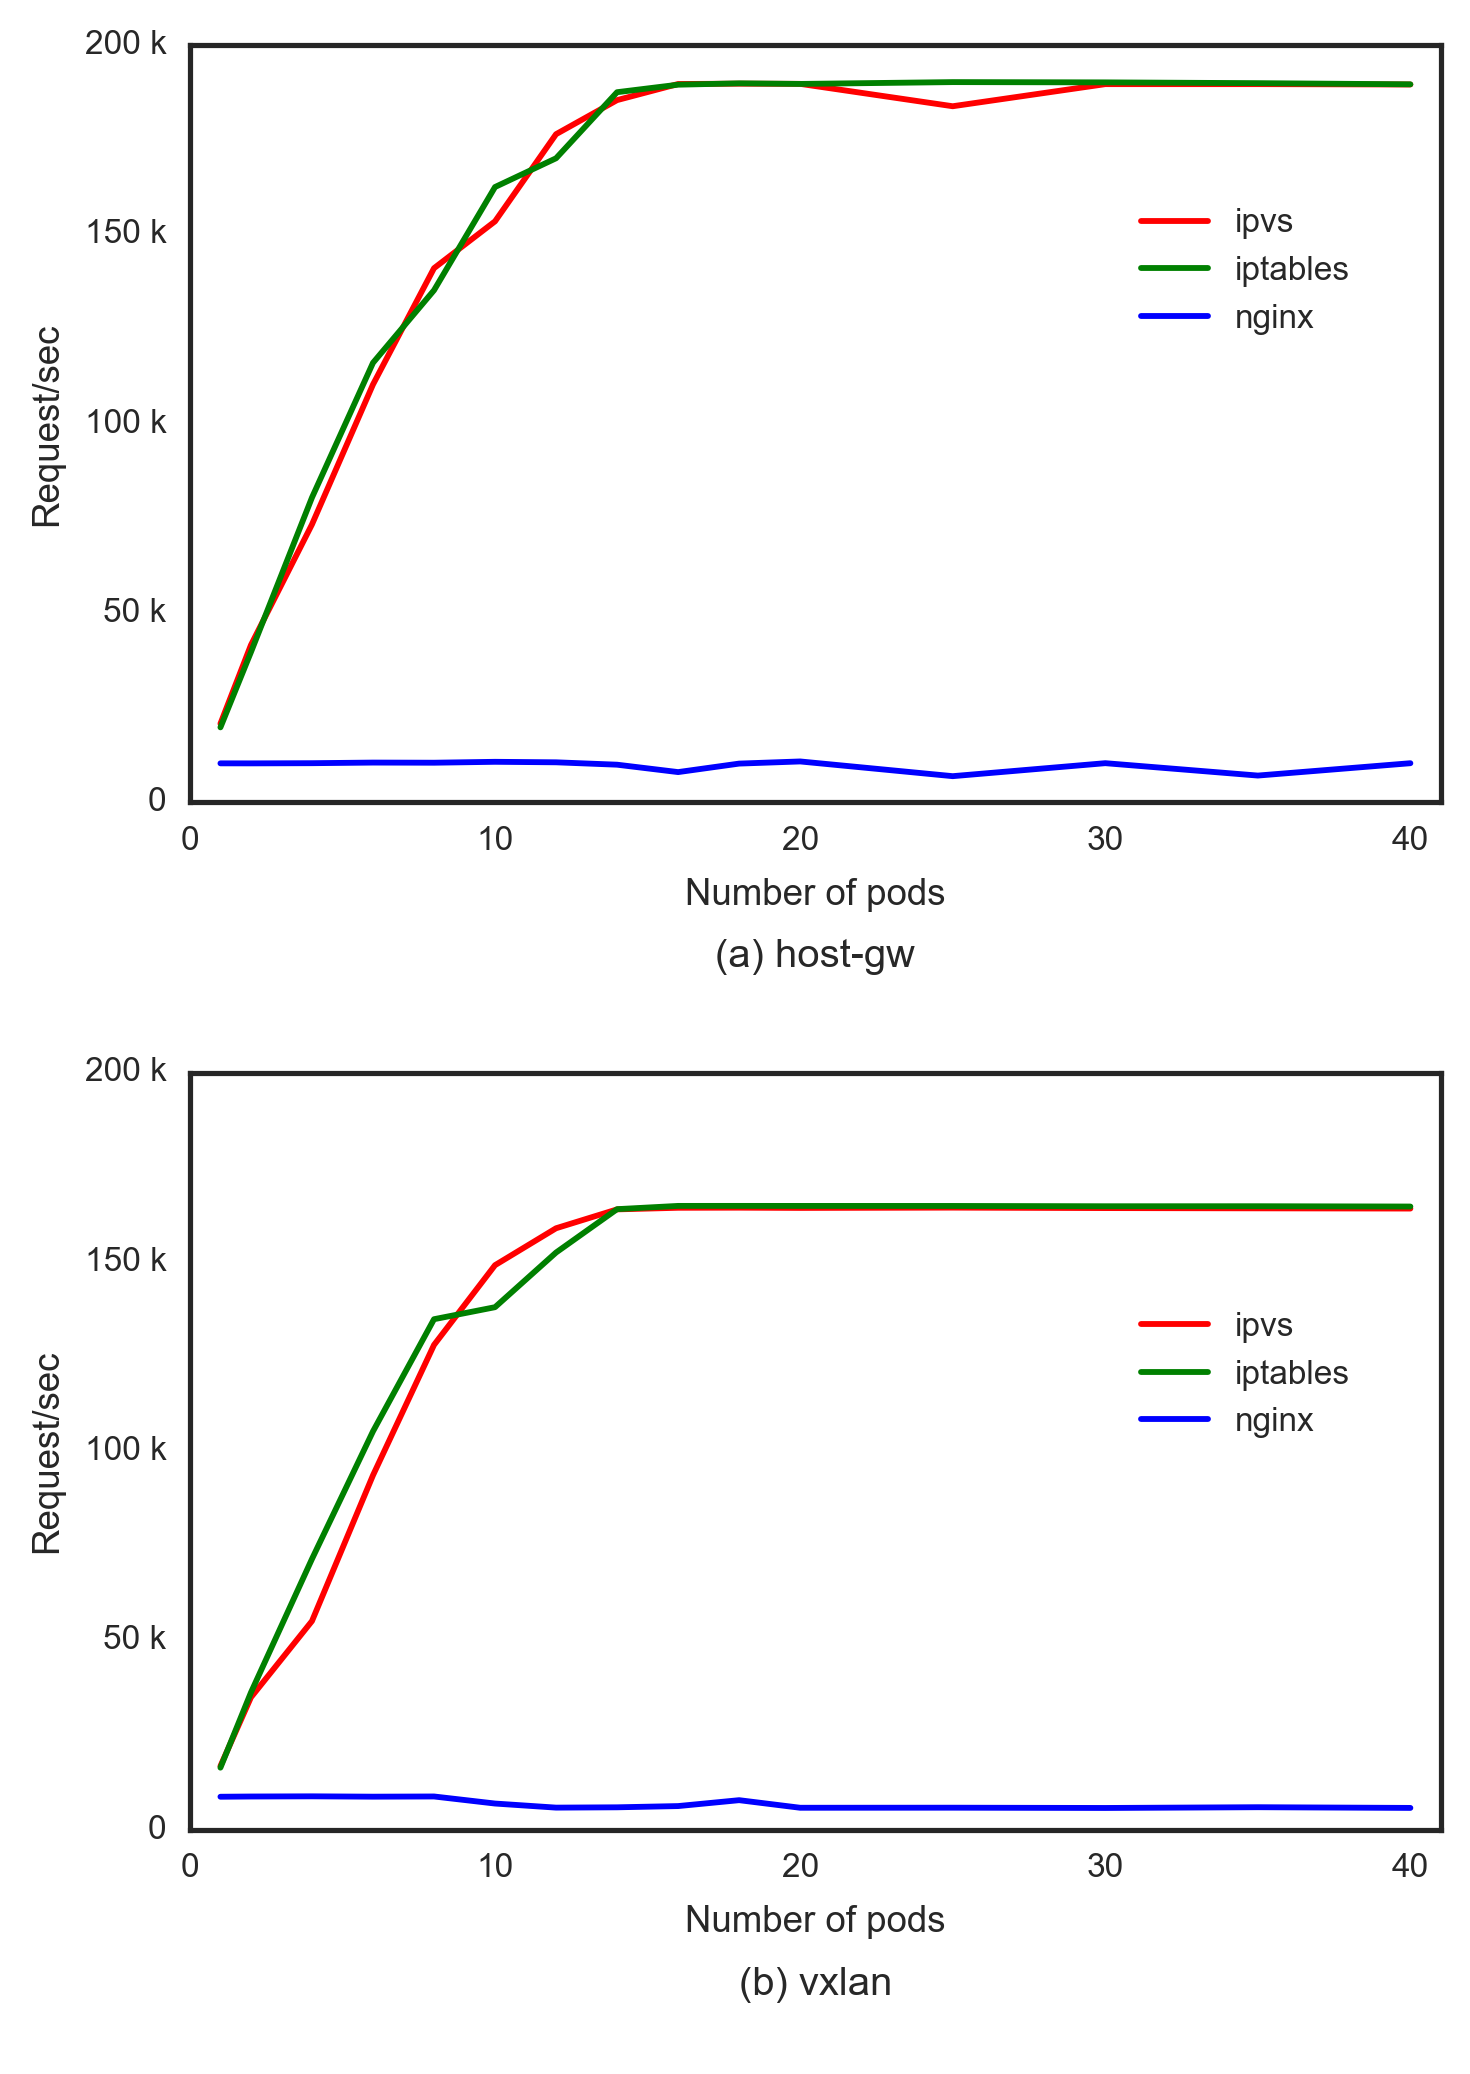
\includegraphics[width=\columnwidth]{Figs/ipvs-iptables-nginx_2figs}
\caption{ipvs and iptables comparison}
\label{fig:ipvs-iptables-nginx_2figs}
\end{figure}



to give these conference by-products a uniform, high-quality
appearance.  To do this, ACM has some rigid requirements for the
format of the proceedings documents: there is a specified format
(balanced double columns), a specified set of fonts (Arial or
Helvetica and Times Roman) in certain specified sizes, a specified
live area, centered on the page, specified size of margins, specified
column width and gutter size.
to give these conference by-products a uniform, high-quality
appearance.  To do this, ACM has some rigid requirements for the
format of the proceedings documents: there is a specified format
(balanced double columns), a specified set of fonts (Arial or
Helvetica and Times Roman) in certain specified sizes, a specified
live area, centered on the page, specified size of margins, specified
column width and gutter size.
to give these conference by-products a uniform, high-quality
appearance.  To do this, ACM has some rigid requirements for the
format of the proceedings documents: there is a specified format
(balanced double columns), a specified set of fonts (Arial or
Helvetica and Times Roman) in certain specified sizes, a specified
live area, centered on the page, specified size of margins, specified
column width and gutter size.
to give these conference by-products a uniform, high-quality
appearance.  To do this, ACM has some rigid requirements for the
format of the proceedings documents: there is a specified format
(balanced double columns), a specified set of fonts (Arial or
Helvetica and Times Roman) in certain specified sizes, a specified
live area, centered on the page, specified size of margins, specified
column width and gutter size.
to give these conference by-products a uniform, high-quality
appearance.  To do this, ACM has some rigid requirements for the
format of the proceedings documents: there is a specified format
(balanced double columns), a specified set of fonts (Arial or
Helvetica and Times Roman) in certain specified sizes, a specified
live area, centered on the page, specified size of margins, specified
column width and gutter size.


\section{Conclusions}\label{Conclusions}
This paragraph will end the body of this sample document.
Remember that you might still have Acknowledgments or
Appendices; brief samples of these
follow.  There is still the Bibliography to deal with; and
we will make a disclaimer about that here: with the exception
of the reference to the \LaTeX\ book, the citations in
this paper are to articles which have nothing to
do with the present subject and are used as
examples only.
%\end{document}  % This is where a 'short' article might terminate


\begin{acks}
  The authors would like to thank Dr. Yuhua Li for providing the
  matlab code of  the \textit{BEPS} method. 

  The authors would also like to thank the anonymous referees for
  their valuable comments and helpful suggestions. The work is
  supported by the \grantsponsor{GS501100001809}{National Natural
    Science Foundation of
    China}{http://dx.doi.org/10.13039/501100001809} under Grant
  No.:~\grantnum{GS501100001809}{61273304}
  and~\grantnum[http://www.nnsf.cn/youngscientsts]{GS501100001809}{Young
    Scientsts' Support Program}.

\end{acks}
